
\documentclass{report}
\usepackage[T1]{fontenc}
\usepackage{ae, aecompl}			% Required for MNRAS
\usepackage{newtxtext, newtxmath} 	% Required for MNRAS
\usepackage{mathtools}
\usepackage{graphicx}
\usepackage{amsmath}
\usepackage{amssymb}
\usepackage{multicol}
\usepackage{bm}
\usepackage{pdflscape}
\usepackage{natbib}
% \usepackage[section]{placeins}
\usepackage{lipsum}
\usepackage{etoolbox}
\usepackage{hyperref}
\usepackage{fancyhdr}
\usepackage[margin = 1in]{geometry}
\hypersetup{
	colorlinks 			= true, 
	urlcolor 			= blue, 
	linkcolor 			= blue, 
	citecolor 			= blue 
}

\newcommand\ddfrac[2]{\frac{\displaystyle #1}{\displaystyle #2}}
\newcommand{\docsdir}{\url{https://github.com/giganano/VICE/tree/master/docs}}

% Journal control sequences defined here because this is a LaTeX report 
% \newcommand{\apj}{ApJ}
% \newcommand{\apjs}{ApJS}
% \newcommand{\aj}{AJ}
% \newcommand{\mnras}{MNRAS}
% \newcommand{\pasa}{PASA}

% \defcitealias{Weinberg2017}{WAF17}

\rfoot{\hyperlink{top}{Back to top}}
\renewcommand{\footrulewidth}{1pt}
\pagestyle{fancy}

\begin{document}
\hypertarget{top}{}
\thispagestyle{empty}
\begin{center}
\underline{\LARGE
	\textbf{\texttt{VICE}: \texttt{Versatile Integrator for Chemical 
	Evolution}}
}
\par\null\par
{\LARGE \textbf{Science Documentation}}
\par\null\par
{\Large \textbf{Version 1.0.0}}
\par\null\par
{\Large
James W. Johnson 
} \par
\textit{The Ohio State University, Department of Astronomy, 140 W. 18th 
Ave., Columbus, OH, 43204}

\par\null\par\noindent
\textbf{\texttt{VICE} is open-source software released under the MIT license. 
We invite researchers and developers to use, modify, and redistribute however 
they see fit under the terms of the associated license. \texttt{VICE}'s source 
code and installation instructions can be found 
at~\url{http://github.com/giganano/VICE.git}. Usage of \texttt{VICE} leading 
to a publication should cite Johnson \& Weinberg (2019, in prep). }

\par\null\par\noindent 
\textit{This documentation is intended to serve neither as a review of 
galactic chemical evolution modeling nor as a means of finding citations on 
previous work in this field. This provides nothing more and nothing less than 
an overview of the numerical implementation of \texttt{VICE} and the analytic 
motivation thereof.}
\end{center}

\par\null\par\noindent 
\underline{\textbf{Quick Links}} 
\par\noindent 
\hyperlink{sec:background}{\textbf{1) Background and Implementation}} 
\par\noindent 
\textbf{2) Single Stellar Populations}
% \hyperlink{sec:ssp}{\textbf{2) Single Stellar Populations}} 
\par
\hyperlink{ssp:lifetimes}{\textbf{2.1) Stellar Lifetimes}} 
\par
\hyperlink{ssp:crf}{\textbf{2.2) The Cumulative Return Fraction}}
\par
\hyperlink{ssp:msmf}{\textbf{2.3) The Main Sequence Mass Fraction}} 
\par
\hyperlink{ssp:enrichment}{\textbf{2.4) Enrichment From Single Stellar 
Populations}} 
\par\noindent 
\textbf{3) The Gas Supply}
% \hyperlink{sec:gas}{\textbf{3) The Gas Supply}} 
\par
\hyperlink{gas:inflows}{\textbf{3.1) Inflows, Star Formation, and Efficiency}}
\par 
\hyperlink{gas:outflows}{\textbf{3.2) Gas Outflows}} 
\par
\hyperlink{gas:recycling}{\textbf{3.3) Recycling}} 
\par\noindent 
\textbf{4) Enrichment}
% \hyperlink{sec:enrichment}{\textbf{4) Enrichment}} 
\par
\hyperlink{enrichment:equation}{\textbf{4.1) The Enrichment Equation}}
\par
\hyperlink{enrichment:ccsne}{\textbf{4.2) Core Collapse Supernovae}} 
\par
\hyperlink{enrichment:sneia}{\textbf{4.3) Type Ia Supernovae}} 
\par
\hyperlink{enrichment:agb}{\textbf{4.4) Asymptotic Giant Branch Stars}} 
\par\noindent 
\textbf{5) Nucleosynthetic Yields}
% \hyperlink{sec:yields}{\textbf{5) Nucleosynthetic Yields}} 
\par
\hyperlink{yields:ccsne}{\textbf{5.1) Core Collapse Supernovae}} 
\par
\hyperlink{yields:sneia}{\textbf{5.2) Type Ia Supernovae}} 
\par
\hyperlink{yields:agb}{\textbf{5.3) Asymptotic Giant Branch Stars}} 
\par
\hyperlink{yields:zscale}{\textbf{5.4) Calibration of the Total Metallicity}}
\par\noindent 
\hyperlink{sec:mdfs}{\textbf{6) Stellar Metallicity Distribution Functions}}
\par\noindent 
\hyperlink{sec:tests}{\textbf{7) Timed Runs}}
\par\noindent 
\hyperlink{sec:figures}{\textbf{8) Figures}}

\vfill
\begin{center}
\textit{
	In this documentation I adopt the notation where $m = M/M_\odot$, a 
	unitless mass measurement relative to the sun. I similarly note $l$ and 
	$u$ as the lower and upper mass limits on star formation, respectively. 
	Deviations from this notation will be made clear by the usage of a capital 
	$M$, meant to denote a mass with dimensionality.  
}
\end{center}
\clearpage


\newpage
\noindent 
\begin{center}
\hypertarget{sec:background}{
	\underline{\LARGE
		\textbf{1) Background and Implementation}
	}
} 
\end{center}
\par\noindent  
\hypertarget{background:gce}{\textbf{1.1) Galactic Chemical Evolution}} 
\par\noindent 
Big Bang Nucleosynthesis only produced hydrogen, helium, and trace amounts of 
lithium, the three lightest elements on the periodic table. Everything else 
is believed to have been produced by various channels of stellar evolution 
and supernovae, the yields of which are dictated by nuclear physics. This has 
an interesting implication for galaxies; being the sites of star formation 
and thus the production of heavy elements in the universe, their chemical 
patterns contain information that is almost if not entirely dependent on their 
formation and evolution through cosmic time. For more information and 
citations thereof, please see section 1 of Johnson \& Weinberg (2019, in prep)
\par\null\par\noindent 
\hypertarget{background:singlezoneapprox}{\textbf{1.2) The Single-Zone 
Approximation}}
\par\noindent 
\texttt{VICE} operates under the single-zone approximation (sometimes also 
referred to as ``box models'', ``one-zone models'', or variations thereof). 
The fundamental assumption of these models is spatial homogeneity in all 
senses of the phrase. The single-zone approximation deliberately sacrifices 
all phase-space information; by assuming that gas, stars, heavy elements, and 
star formation efficiency is distributed uniformly, the need for N-body or 
hydro simulations is eliminated. This reduces the associated equations to a 
system of coupled integro-differential equations with time, which are easily 
integrated numerically. Mild numerical approximations often yield analytic 
results in some cases. This drastically reduces the computational expense 
associated with the galactic chemical evolution. For more information and 
citations thereof, please see sections 1 and 2 of Johnson \& Weinberg, (2019, 
in prep). 
\par\null\par\noindent 
\hypertarget{background:implementation}{\textbf{1.3) Implementation}}
\par\noindent 
\texttt{VICE} is capable of simulating the enrichment of and calculating 
nucleosynthetic yields for 76 astrophysically produced elements. This includes 
all elements between carbon and bismuth with the exceptions of technetium and 
promethium (atomic numbers 43 and 61), whose isotopes are all radioactive. 
\texttt{VICE}'s primary motivation is to model the enrichment of these 
elements in galaxies over cosmic time, simulating enrichment from core-collapse 
supernovae, type Ia supernovae, and asymptotic giant branch stars. In it's 
current version, it does not model enrichment via the r-process or merging 
neutron stars in any way. 
\par
In this documentation, I outline the numerical approximations implemented in 
\texttt{VICE}; they constitute a solution to the equations of the single-zone 
approximation as an initial value problem via Euler's method. While Euler's 
method is known to have the largest errors associated with numerical 
calculations, this is not of concern for \texttt{VICE}, because the models 
built into this software carry intrinsic errors at the~$\sim$10\% level. Thus 
numerical artifacts are not the dominant sources of error. 
\par
In solving for the abundances of various elements under the single-zone 
approximation, Euler's method also allows each timestep to be modeled as a 
simple stellar population. Because more sophisticated timestep algorithms 
require information at fractions of timesteps, this approach is made possible 
by Euler's method alone. While simplifying the numerical algorithm 
intrinsically, this also allows integrals over the simulated galaxy's history 
to transform into simple summations over all previous timesteps. In this 
manner, the adoption of Euler's method allows \texttt{VICE} to achieve 
powerful computing speeds. 
\par
Furthermore, \texttt{VICE}'s timestep algorithms are implemented entirely in 
\texttt{ANSI/ISO C}, allowing it to reach computing speeds simply not allowed 
by a pure \texttt{python} implementation. These functions are wrapped in 
\texttt{Cython} so that they may be called from a \texttt{python} interpreter. 
With implementation purely in standard library \texttt{C} and \texttt{python}, 
\texttt{VICE} is entirely cross platform and totally independent of the user's 
version of \texttt{anaconda} (or lackthereof). However, \texttt{VICE} is 
simply not wrapped for installation on Windows operating systems, and users 
will not be able to install \texttt{VICE} on a Windows machine without hacking 
the installation source code. For this reason, the authors do not offer support 
for users who have installed \texttt{VICE} on Windows. 


\newpage
\noindent 
\begin{center}
\hypertarget{ssp:lifetimes}{
	\underline{\LARGE
		\textbf{2.1) Stellar Lifetimes}
	}
}
\end{center}
I adopt in \texttt{VICE} the commonly used approximation for the lifetime of 
a star on the main sequence: 
\begin{equation}
\tau_\text{MS} \approx (10\text{ Gyr})m^{-3.5}
\end{equation}
where 10 Gyr is the assumed lifetime of the sun on the main sequence. The 
scaling of $\tau_\text{MS}\sim m^{-3.5}$ fails for high mass 
($\gtrsim8M_\odot$) stars, but these stars have lifetimes that are very short 
compared to the relevant timescales of galactic chemical evolution ($\sim$few 
Myr compared to~$\sim$few Gyr). This approximation fails for low mass stars as 
well ($\lesssim0.5M_\odot$), but these stars have such long lifetimes that 
none of them have evolved off of the main sequence over the entire lifetime of 
the universe. Because the relevant timescales for galactic chemical evolution 
are a few to 10 Gyr, it is the intermediate mass stars with lifetimes on this 
order of magnitude that need to be modeled properly. 
\par 
By interpreting $\tau_\text{MS}$ as the age of a stellar population $t$, this 
equation can be inverted to solve for the turnoff mass $m_\text{to}(t)$ - the 
mass of stars that are evolving off of the main sequence: 
\begin{equation}
m_\text{to}(t) = \Big(\frac{t}{10\text{ Gyr}}\Big)^{-1/3.5}
\end{equation}
With the manner in which \texttt{VICE} is implemented, the turnoff mass is 
a much more numerically convenient quantity than the main sequence lifetimes 
of stars, because it is invoked in both the cumulative return 
fraction (section~\hyperlink{ssp:crf}{2.2}) and the main sequence mass 
fraction (section~\hyperlink{ssp:msmf}{2.3}). Source code can be found 
at~\url{https://github.com/giganano/VICE/blob/master/vice/src/recycling.c}. 






%------------------------- cumulative return fraction ------------------------% 
\newpage
\noindent
\begin{center}
\hypertarget{ssp:crf}{
	\underline{\LARGE
		\textbf{2.2) The Cumulative Return Fraction}
	}
}
\end{center}
\par\noindent 
I define the cumulative return fration as the fraction of a single stellar 
population's (or star cluster's) mass that is returned to the interstellar 
medium (ISM) as gas at the birth metallicity of the stars. As stars evolve off 
the main sequence, leaving behind a remnant, whatever mass does not end up in 
the remnant is returned to the ISM. This quantity varies with time and is thus 
denoted here accordingly as $r(t)$, where $t$ is the star cluster's age. In 
this section, I consider only the total mass that is returned to the ISM. The 
impact of recycling on enrichment in detailed in 
section~\hyperlink{enrichment:equation}{4.1}. I demonstrate here that this 
quantity is uniquely specified by the adopted stellar initial mass function 
(IMF), the lifetimes of stars on the main sequence as a function of mass, and 
the mass of stellar remnants left behind also a function of mass. Its full 
analytic expression is given by: 
\begin{equation}
r(t) = \ddfrac{
	\int_{m_\text{to}(t)}^u (m - m_\text{rem})\frac{dN}{dm}dm
}{
	\int_l^u m\frac{dN}{dm}dm
}
\end{equation}
The numerator is an integral over the stellar IMF from the \textit{turnoff 
mass} $m_\text{to}$ to the upper mass limit of star formation $u$ weighted by 
the mass of these stars that does not end up in the remnant. The denominator 
is also an integral over the stellar IMF, but instead over the entire mass 
range for star formation $l$ to $u$ weighted by the initial mass of the stars 
$m$. This is nothing more than a mathematical statement of ``ejected gas from 
dead stars over the sum total mass of all of them''. 
\par
\texttt{VICE} adopts the model of Kalirai et al. (2008), ApJ, 676, 594, where 
the remnant mass is specified by: 
\begin{equation}
M_\text{rem} = 
\begin{dcases}
1.44 M_\odot & (M \geq 8 M_\odot) \\ 
0.394 M_\odot + 0.109 M & (M < 8 M_\odot)
\end{dcases}
\end{equation}
I derive the following expression given a power law IMF 
$dN/dm \propto m^{-\alpha}$ for the numerator of $r(t)$: 
\begin{equation}\begin{split}
\int_{m_\text{to}}^u (m - m_\text{rem})\frac{dN}{dm}dm = 
\frac{
	1
}{
	2 - \alpha
} m^{2 - \alpha}\Big|_{m_\text{to}(t)}^u  - 
\begin{dcases} 
\frac{1.44}{1 - \alpha}m^{1 - \alpha}\Big|_{m_\text{to}(t)}^u & 
(m_\text{to}(t) \geq 8) \\ 
\frac{1.44}{1 - \alpha}m^{1 - \alpha}\Big|_8^u + \Big[
\frac{0.394}{1 - \alpha}m^{1 - \alpha} + \frac{0.109}{2 - \alpha}m^{2 - \alpha}
\Big]_{m_\text{to}(t)}^8 & 
(m_\text{to}(t) < 8)
\end{dcases}
\end{split}\end{equation}
This solution is analytic, and thus without any numerical approximations. For 
piecewise IMFs, this becomes a summation over the relevant mass ranges of the 
IMF where each term has the exact same form. The normalization of the IMF is 
irrelevant, because the same normalization appears in the denominator, and 
they thus cancel. 
\par 
Also for a power law IMF with index $\alpha$, I derive the following 
expression for the denominator of $r(t)$: 
\begin{equation}
\int_l^u m\frac{dN}{dm}dm = \frac{1}{2 - \alpha}m^{2 - \alpha}\Big|_l^u
\end{equation}
\par
Weinberg, Andrews \& Freudenburg (2017), ApJ, 837, 183 adopted 
instantaneous recycling, whereby a given fraction of a single stellar 
population's mass is returned to the ISM at the same metallicity 
instananeously. They demonstrated that $r_\text{inst}$ = 0.2 and 
$r_\text{inst}$ = 0.4 are good approximations for the 
Salpeter\footnote{
	Salpeter (1955), ApJ, 121, 161
} and Kroupa\footnote{
	Kroupa (2001), MNRAS, 322, 231 
} IMFs. This reduces the more sophisticated formulation detailed here to 
\begin{equation}
r(t) \approx 
\begin{dcases} 
r_\text{inst} & (t = 0) \\ 
0 & (t \neq 0)
\end{dcases} 
\end{equation}
\par
\texttt{VICE} gives users the ability to specify an instantaneous recycling 
parameter, but implements continuous recycling by default. This is done 
self-consistently given the user's specified IMF and lower and upper mass 
limits on star formation. Source code for the implementation of recycling and 
the cumulative return fraction can be found 
at~\url{https://github.com/giganano/VICE/blob/master/vice/src/recycling.c}. 
\par
I plot $r(t)$ as a function of time for both Kroupa and Salpeter IMFs in 
figure~\ref{fig:rh_2panel}. The offset between the two IMFs is due to the 
difference in the number of low mass stars as predicted by the two IMFs. 





% ------------------------- main sequence mass fraction ----------------------% 
\newpage 
\noindent
\begin{center} 
\hypertarget{ssp:msmf}{
	\underline{\LARGE
		\textbf{2.3) The Main Sequence Mass Fraction}
	}
}
\end{center}
\par\noindent 
I define the main sequence mass fraction as the fraction of a single 
stellar population's mass that is still in the form of main sequence stars. 
I denote this quantity as $h(t)$\footnote{
	$h$ rather than $m$ since $m$ already denotes mass. I choose $h$ for 
	hydrogen fusion in the cores of these stars. 
}, where $t$ is the star cluster's age. I demonstrate that this quantity is 
uniquely specified by the adopted stellar initial mass function (IMF) and 
the lifetimes of stars on the main sequence. It's analytic expression is given 
by: 
\begin{equation}
h(t) = \ddfrac{
	\int_l^{m_\text{to}(t)} m\frac{dN}{dm}dm 
}{
	\int_l^u m\frac{dN}{dm}dm
}
\end{equation}
Both the numerator and the denominator are mass-weighted integrals over the 
IMF, but the numerator does not count evolved stars. This is purely a 
mathematical statement of ``main sequence mass over initial mass.'' 
\par 
For a power law IMF $dN/dm \propto m^{-\alpha}$, 
\begin{equation}
h(t) = \ddfrac{
	\frac{1}{2 - \alpha}m^{2 - \alpha}\Big|_l^{m_\text{to}(t)}
}{
	\frac{1}{2 - \alpha}m^{2 - \alpha}\Big|_l^u
}
\end{equation}
It may be tempting to cancel the factor of $1/2 - \alpha$, but much more 
careful considerations must be taken for piece-wise IMFs like Kroupa\footnote{
	Kroupa (2001), MNRAS, 322, 231 
}. 
\begin{equation}
h(t) \rightarrow \ddfrac{
	\Big[\sum_i\frac{1}{2 - \alpha_i} m^{2 - \alpha_i}\Big]_l^{m_\text{to}(t)}
}{
	\Big[\sum_i\frac{1}{2 - \alpha_i} m^{2 - \alpha_i}\Big]_l^u 
}
\end{equation}
where the summation is over the relevant piece-wise mass ranges. 
\par
\texttt{VICE} currently onlow allows functionality for the Kroupa and 
Salpeter\footnote{
	Salpeter (1955), ApJ, 121, 161
} IMFs. In the case of the Kroupa IMF, $\alpha$ = 0.3 [1.3] [2.3] for stellar 
masses in the range $\leq$ 0.08$M_\odot$ [$0.08M_\odot \leq M \leq 0.5M_\odot$] 
[$\geq 0.5M_\odot$]. For Salpeter, $\alpha$ = 2.35 for all stellar masses. 
\par
\texttt{VICE} implements the main sequence mass fraction self-consistently 
given the user's specified stellar IMF. Source code can be found 
at~\url{https://github.com/giganano/VICE/blob/master/vice/src/recycling.c}. 
\par
I plot $h(t)$ in the right-hand panel of Figure~\ref{fig:rh_2panel} for 
both Kroupa and Salpeter initial mass functions. The offset between the two is 
due to the difference in the number of low mass stars as predicted by the 
two IMFs. As discussed in section~\hyperlink{enrichment:agb}{4.4}, 
$h(t) \approx 1 - r(t)$ fails at the~$\sim$15\% level for single stellar 
populations at late times due to the masses of stellar remnants. For this 
reason, the recycling fraction is not used in determing the rate of enrichment 
from AGB stars. 





\newpage 
\noindent 
\begin{center}
\hypertarget{ssp:enrichment}{
	\underline{\LARGE 
		\textbf{2.4) Enrichment from Single Stellar Populations} 
	}
}
\end{center}
While galaxies form stars continuously, sometimes astronomers are interested 
in the enrichment patterns of individual stellar populations. This is 
inherently cheaper computationally, since this is only one stellar population 
while a galaxy simulation would take into account multiple stellar populations. 
\par
\texttt{VICE} includes functionality for simulating the mass production of a 
given element from a single stellar population (i.e. an individual star 
cluster) of given mass and metallicity under their adopted yields. This by 
construction does not take into account depletion from infalling low 
metallicity gas and star formation, ejection in outflows, recycling, etc. It 
only calculates the mass of the element produced as a function of time. 
\par
At time $t = 0$, there is no mass produced, because this is adopted as the 
time at which the star cluster forms. Because \texttt{VICE} operates under 
the assumption that all core-collapse supernovae happen instantaneously, at 
$t = \Delta t$, the entire core-collapse nucleosynthetic yield is injected: 
\begin{equation}
\Delta M_x = y_x^\text{CC}(Z)M_*
\end{equation}
where $y_x^\text{CC}(Z)$ is the user's current yield setting for core collapse 
supernovae at the metallicity of the stars $Z$. At subsequent timesteps, 
enrichment from asymptotic giant branch stars: 
\begin{equation} 
\dot{M}_x^\text{AGB}\Delta t \approx y_x^\text{AGB}(m_\text{to}(t) | Z) 
M_* [h(t) - h(t + \Delta t)]
\end{equation}
and type Ia supernovae: 
\begin{equation}
\dot{M}_x^\text{Ia}\Delta t \approx y_x^\text{Ia}M_*\ddfrac{
	R_\text{Ia}(t)
}{
	\int_0^\infty R_\text{Ia}(t')dt'
}
\end{equation}
are injected. For details on these equations, see 
sections~\hyperlink{enrichment:ccsne}{4.2} 
(CCSNe),~\hyperlink{enrichment:sneia}{4.3} (SNe Ia) 
and~\hyperlink{enrichment:agb}{4.4} (AGB stars). These are the same equations 
that are implemented in simulating enrichment under the single-zone 
approximation, but applied to only one episode of star formation. 
\par
Users can run these simulations directly by calling 
\texttt{vice.single\_stellar\_population}. Python wrapping for this function 
can be found 
at~\url{https://github.com/giganano/VICE/blob/master/vice/core/_wrapper.pyx}, 
with source code 
at~\url{https://github.com/giganano/VICE/blob/master/vice/src/metals.c}. 









%----------------------------- The Gas Supply --------------------------------%
\newpage 
\noindent 
\begin{center}
\hypertarget{gas:inflows}{
	\underline{\LARGE
		\textbf{3.1) Inflows, Star Formation, and Efficiency}
	}
}
\end{center}
\par\noindent 
For a spatially homogeneous cloud of gas with mass infall rate (IFR) 
$\dot{M}_\text{in}$, star formation rate (SFR) $\dot{M}_*$, and outflow rate 
(OFR) $\dot{M}_\text{out}$, the time-derivative of the mass of the ISM gas is 
given by: 
\begin{equation}
\label{eq:mgdot}
\dot{M}_\text{g} = \dot{M}_\text{in} - \dot{M}_* - \dot{M}_\text{out} + 
\dot{M}_\text{r} 
\end{equation}
where $\dot{M}_\text{r}$ is the rate of recycling from stars evolving off of 
the main sequence and returning gas to the ISM at their birth metallicity. 
Equation~\ref{eq:mgdot} is approximated numerically in the following manner: 
\begin{equation}
\Delta M_\text{g} \approx \dot{M}_\text{g}\Delta t = \dot{M}_\text{in}\Delta t 
- \dot{M}_*\Delta t - \dot{M}_\text{out}\Delta t + \dot{M}_\text{r}\Delta t
\end{equation}

\par\null\par\noindent 
By construction, \texttt{VICE} operates such that the user specifies either an 
infall history ($\dot{M}_\text{in}$ as a function of time), a star formation 
history ($\dot{M}_*$ as a function of time), or the gas history ($M_\text{g}$ 
as a function of time). The user also specifies a star formation efficiency 
prescription: 
\begin{equation}
\tau_* \equiv M_\text{g} / \dot{M}_*
\end{equation} 
$\tau_*$ can be any arbitrary function of time that the user has coded into 
\texttt{python}, allowing simulation of star formation efficiency prescriptions 
of arbtirary complexity. With one of either $\dot{M}_\text{in}$, $\dot{M}_*$, 
or $M_\text{g}$ specified by the user, $\tau_*$, and the implementation of 
$\dot{M}_\text{out}$ and $\dot{M}_\text{r}$ detailed in 
sections~\hyperlink{gas:outflows}{3.2} and~\hyperlink{gas:recycling}{3.3}, the 
solution to equation~\ref{eq:mgdot} is unique. 
\par
\texttt{VICE}'s \texttt{singlezone} timestep integrator provides users a 
switch with which they can turn on gas-dependent star formation efficiency. 
In accordance with the Kennicutt-Schmidt relation, this is implemented as a 
power law: 
\begin{equation}
\tau_*^{-1}(t) = \tau_{*,\text{spec}}^{-1}(t)\Big(\frac{
	M_\text{g}
}{
	M_\text{g,Schmidt}
}\Big)^\texttt{schmidt\_index}
\end{equation}
where $M_\text{g}$ is the gas supply at any given timestep, and 
$M_\text{g,Schmidt}$ and \texttt{schmidt\_index} are user-specified model 
parameters built into the \texttt{singlezone} class. When a \texttt{singlezone} 
object's attribute \texttt{schmidt} = \texttt{True}, the user-specified 
$\tau_*$ is treated as $\tau_{*,\text{spec}}$ in the above equation. See 
\texttt{vice.singlezone.tau\_star} in the user's guide for more information.  
\par
Source code for the implementation of these equations in \texttt{VICE} can 
be found at~\url{https://github.com/giganano/VICE/blob/master/vice/src/metals.c}. 





\newpage
\noindent 
\begin{center}
\hypertarget{gas:outflows}{
	\underline{\LARGE
		\textbf{3.2) Gas Outflows} 
	}	
}
\end{center}
\par\noindent 
Most galactic chemical evolution models adopt a dimensionless parameter known 
as the \textit{mass loading factor}, which quantifies the strength of 
galactic winds as the ratio of the outflow rate to the star formation 
rate $\eta \equiv \dot{M}_\text{out}/\dot{M}_*$. In Johnson \& Weinberg 
(2019), we introduced a new parameter into single-zone galactic chemical 
evolution modeling in an attempt to generalize this relationship, which we 
dubbed the \textit{smoothing time}. This is the timescale on which the 
star-formation rate is averaged (or ``smoothed'') to determine the outflow 
rate: 
\begin{equation}\begin{split}
\dot{M}_\text{out} &= \eta(t)\langle\dot{M}_*\rangle_{\tau_\text{s}} \\ 
&= \begin{dcases} 
\frac{\eta(t)}{\tau_\text{s}}\int_{t - \tau_\text{s}}^t \dot{M}_*(t')dt' & 
(t \geq \tau_\text{s}) \\ 
\frac{\eta(t)}{t}\int_0^t \dot{M}_*(t')dt' & (0 \leq t \leq \tau_\text{s}) 
\end{dcases} 
\end{split}\end{equation}
Under this formulation, the expression is piece-wise to ensure no numerical 
artifacts are introduced by smoothing over the star formation history 
evaluated from a negative timestep. \texttt{VICE} implements the following 
numerical approximation: 
\begin{equation}
\dot{M}_\text{out} = 
\begin{dcases} 
\eta(t)\frac{\Delta t}{\tau_\text{s}}\sum_{i = 0}^{\tau_\text{s}/\Delta t} 
\dot{M}_*(t - i\Delta t) & (t \geq \tau_\text{s}) \\ 
\eta(t)\frac{\Delta t}{t}\sum_{i = 0}^{t/\Delta t}\dot{M}_*(t - i\Delta t) & 
(0 \leq t \leq \tau_\text{s})
\end{dcases}
\end{equation} 
In words, at each timestep \texttt{VICE} simply looks back the number of 
timesteps corresponding to the smoothing time, and determines the arithmetic 
mean of the star formation rate over those timesteps. An advantage of this 
formulation is that when $\tau_\text{s} < \Delta t$, \texttt{VICE} 
automatically recovers the traditional relation 
$\dot{M}_\text{out} = \eta(t)\dot{M}_*(t)$. 
\par
The mass loading parameter is a user-specified function of time. By 
implementing $\eta(t)$ in this manner, \texttt{VICE} achieves the capability 
of simulation galaxies with arbitrarily complex mass loading factors. I 
clarify that it is only the star formation rate which is time-averaged under 
this formulation; the user-specified $\eta(t)$ is taken to be an 
instantaneous function. 
\par
Source code can be found 
at~\url{https://github.com/giganano/VICE/blob/master/vice/src/metals.c}. 



\newpage
\noindent 
\begin{center}
\hypertarget{gas:recycling}{
	\underline{\LARGE
		\textbf{3.3) Recycling} 
	}
}
\end{center}
\par\noindent 
As stars evolve off of the main sequence, the mass that does not end up in the 
remnant is returned to the interstellar medium. The net effect of this from 
all previous episodes of star formation quantifies the rate of mass recycling. 
\begin{equation}
\dot{M}_\text{r} = \int_0^t \dot{M}_*(t - t')\frac{dr(t')}{dt}dt 
\end{equation} 
where $r(t')$ is the cumulative return fraction (see 
section~\hyperlink{ssp:crf}{2.2} for details). Obtaining the cumulative return 
fraction itself is somewhat more feasible than its time derivative. For this
reason, I approximate the total mass recycled in a given timestep in the 
following manner. 
\begin{equation}
\label{eq:mdotr}
\Delta M_\text{r} \approx\dot{M}_\text{r}\Delta t = 
\sum_{i = 0}^{t/\Delta t}\dot{M}_*(t - i\Delta t)[r((i + 1)\Delta t) - 
r(i\Delta t)]\Delta t
\end{equation}
This is easier and thus faster computationally since $r(t)$ is calculated 
numerically at the beginning of each \texttt{VICE} integration. Because 
$\dot{M}_*\Delta t$ is simply the initial mass of the stellar population that 
forms at some timestep, this summation is simply adding up the fractional 
changes in mass from each previous timestep and returning it to the ISM gas.
\par
\texttt{VICE} also allows users to pass an instantaneous recycling parameter 
$r_\text{inst}$, in which case the recycled mass is simply: 
\begin{equation}
\dot{M}_\text{r}\Delta t \approx r_\text{inst}\dot{M}_*\Delta t
\end{equation}
Weinberg, Andrews \& Freudenburg (2017), ApJ, 837, 183 found that this is a 
good approximation, with $r_\text{inst} \approx 0.4\ (0.2)$ for a Kroupa 
(Salpeter) IMF as recommended values. 
\par 
This is how recycling is implemented numerically in \texttt{VICE}. By default, 
it will adopt the continuous recycling prescription of equation~\ref{eq:mdotr}. 
Source code can be found 
at~\url{https://github.com/giganano/VICE/blob/master/vice/src/recycling.c}. 

\par 


% \newpage 
% \noindent 
% \begin{center} 
% \hypertarget{gas:inflow}{
% 	\underline{\LARGE
% 		\textbf{3.1) Gas Inflow}
% 	}
% }
% \end{center}
% \par\noindent 
% \texttt{VICE} allows users to specify a mass inflow rate that is an arbitrary 
% function of time. It must take only one parameter, which \texttt{VICE} will 
% interpret as time in Gyr. \texttt{VICE} interprets the returned value as the 
% mass infall rate of intergalactic gas onto the galaxy in $M_\odot$ yr$^{-1}$. 
% To do so, users should create an instance of the \texttt{vice.singlezone} 
% class, make sure that its attribute \texttt{mode} = \texttt{``ifr''}, and 
% pass their preferred function to the attribute \texttt{func}. 
% \par 
% \texttt{VICE} also allows users to specify a callable function of time for the 
% infall metallicity of each individual element. The \texttt{singlezone} class 
% has an attribute \texttt{zin}, which the user can set to a 
% \texttt{VICE dataframe} relating each element to a user-constructed function 
% of time. 









%-------------------------------- Enrichment --------------------------------% 
% \newpage
% \noindent 
% \begin{center} 
% \hypertarget{sec:enrichment}{
% 	\underline{\LARGE
% 		\textbf{4) Enrichment}
% 	}
% }
% \end{center}









%-------------------------- The Enrichment Equation --------------------------% 
\newpage 
\noindent 
\begin{center} 
\hypertarget{enrichment:equation}{
	\underline{\LARGE
		\textbf{4.1) The Enrichment Equation} 
	}
}
\end{center}
\par\noindent 
For an arbitrary element $x$ on the periodic table, the enrichment equation 
has the following general form: 
\begin{equation}
\dot{M}_x = \dot{M}_x^\text{CC} + \dot{M}_x^\text{Ia} + \dot{M}_x^\text{AGB} 
- \frac{M_x}{M_\text{g}}[\dot{M}_* + \xi_\text{enh}\dot{M}_\text{out}] + 
\dot{M}_x^\text{r} + Z_\text{x,in}\dot{M}_\text{in}
\end{equation}
This equation is nothing than a mathematical statement that at any given time 
(from left to right on the right-hand side), the element $x$ is enriched via 
core-collapse supernovae (CCSNe), type Ia supernovae (SNe Ia), and asymptotic 
giant branch (AGB) stars. Simultaneously, it is depleted due to star formation 
at the current metallicity of the interstellar medium (ISM) $M_x/M_\text{g}$ 
and outflows at some multiplicative factor $\xi_\text{enh}$ above or below the 
ISM metallicity.  It is also re-enriched due to recycling from previous 
generations of stars and inflows of some metallicity $Z_\text{x,in}$.  
\par
I detail the $\dot{M}_x^\text{CC}$, $\dot{M}_x^\text{Ia}$, and 
$\dot{M}_x^\text{AGB}$ terms individually, and the rest of them here. Source 
code for the implementation of this equation in \texttt{VICE} can be found 
at~\url{https://github.com/giganano/VICE/blob/master/vice/src/metals.c}. 
\par
\texttt{VICE} operates under the assumption that star formation occurs at the 
current metallicity of the ISM $M_x/M_\text{g}$. Hence the 
$-(M_x/M_\text{g})\dot{M}_*$ sink term in the enrichment equation. 
\par 
Many galactic chemical evolution models have operated under the assumption that 
outflows occur at or near the metallicity of the ISM (i.e. 
$\dot{M}_x^\text{out} \approx (M_x/M_\text{g})\dot{M}_\text{out}$). However, 
recent work in the literature from both simulations (e.g. Christensen et al. 
(2018), ApJ, 867, 142) and observations (e.g. Chisholm, Tremonti \& Leitherer 
(2018), MNRAS, 481, 1690) have suggested that this may not be the case. 
Therefore, \texttt{VICE} allows outflows to occur at some multiplicative 
factor of the ISM metallicity, which may vary with time. Hence the 
$(M_x/M_\text{g})\xi_\text{enh}\dot{M}_\text{out}$ sink term in the enrichment 
equation. 
\par 
At any given time, there will be nonzero metallicity stars returning gas to 
the ISM at their birth metallicity. This is mathematically similar to the rate 
of gas recycling as discussed in section~\hyperlink{gas:recycling}{3.3}, but 
weighted by the metallicities of the stars. Since \texttt{VICE} operates under 
the assumption that star formation occurs at the metallicity of the ISM: 
\begin{equation}\begin{split}
\dot{M}_x^\text{r} &= \int_0^t \dot{M}_*(t - t')Z_x^\text{ISM}(t - t')
\frac{dr(t')}{dt}dt \\
\dot{M}_x^\text{r}\Delta t &\approx \sum_{i = 0}^{t/\Delta t}
\dot{M}_*(t - i\Delta t)Z_x^\text{ISM}(t - i\Delta t)
[r((i + 1)\Delta t) - r(i\Delta t)]\Delta t
\end{split}\end{equation}
In the event that the user has specified instantaneous recycling, this 
equation simplifies: 
\begin{equation}
\dot{M}_x^\text{r}\Delta t \approx r_\text{inst}\dot{M}_*Z_x^\text{ISM}\Delta t
\end{equation} 
Source code for the recycling rate can found 
at~\url{https://github.com/giganano/VICE/blob/master/vice/src/recycling.c}. 
\par
At any given timestep, there is gas infall onto galaxies of a given metallicity 
$Z$. This introduces a $Z_\text{x,in}\dot{M}_\text{in}$ term into the 
enrichment equation quantifying the addition of a given element $x$ due to 
metal-rich infall. \texttt{VICE} allows users to specify a function of time 
$Z_\text{x,in}$ for each individual element. In this manner, \texttt{VICE} 
supports simulations of metal-rich infall with full generality. Source code 
for this feature can be found in the source code for the \texttt{singlezone} 
class, available 
at~\url{https://github.com/giganano/VICE/blob/master/vice/core/_wrapper.pyx}. 






%----------------------------------- CCSNe -----------------------------------% 
\newpage 
\noindent 
\begin{center} 
\hypertarget{enrichment:ccsne}{
	\underline{\LARGE
		\textbf{4.2) Core Collapse Supernovae} 
	}
}
\end{center}
\par\noindent 
Core collapse supernovae (CCSNe) are the explosions of massive stars 
($\gtrsim8M_\odot$) at the end of the nuclear lifetimes. Due to the steep 
nature of the lifetime-stellar mass relationship, these stars have lifetimes 
that are extremely short compared to the relevant timescales of galactic 
chemical evolution ($\sim$few Myr compared to~$\sim$few Gyr). This means that, 
to an extremely good approximation, the lifetimes of these stars can be 
treated as instantaneous in galactic chemical evolution models. The enrichment 
from CCSNe thus instantaneously converts some fraction of a single stellar 
population's mass into a given element $x$ under this approximation, implying 
a linear relationship between the rate of mass enrichment and the 
star formation rate: 
\begin{equation}
\dot{M}_x^\text{CC} = y_x^\text{CC}(Z)\dot{M}_* 
\end{equation}
where $y_x^\text{CC}(Z)$ is the fraction of the stellar population's mass 
which is converted to the element $x$, which may be dependent on the 
metallicity $Z$. This is the IMF-integrated fractional nucleosynthetic yield 
of the element $x$ from CCSNe; see section~\hyperlink{yields:ccsne}{5.1} for 
more information on this quantity. 
\par
Source code for the implementation of this equation in \texttt{VICE} can be 
found at~\url{https://github.com/giganano/VICE/blob/master/vice/src/ccsne.c}. 





%---------------------------------- SNe Ia ----------------------------------% 
\newpage
\noindent 
\begin{center} 
\hypertarget{enrichment:sneia}{
	\underline{\LARGE
		\textbf{4.3) Type Ia Supernovae} 
	}
}
\end{center}
\par\noindent 
Type Ia supernovae (SNe Ia) are the thermonuclear detonations of white dwarf 
(WD) stars. Being the remnants of lower mass stars, WDs are produced on longer 
timescales than CCSNe; this requires an intrinsic delay-time distribution (DTD) 
$R_\text{Ia}$ to accurately model this channel of enrichment. 
\par
I define the SNe Ia DTD as the rate of SNe Ia explosions associated with only 
one stellar population. A time $t$ following the formation of a single stellar 
population, the rate of enrichment of an element $x$ is given by the normalized 
rate of SNe Ia: 
\begin{equation}
\dot{M}_x^\text{Ia} = y_x^\text{Ia}M_* \ddfrac{
	R_\text{Ia}(t)
}{
	\int_0^\infty R_\text{Ia}(t')dt'
}
\end{equation}
\texttt{VICE} allows users to specify any arbitrary function of time as 
$R_\text{Ia}(t)$. It also has built-in functionality for exponential DTDs 
($R_\text{Ia} \propto e^{-t/\tau_\text{Ia}}$ for some $\tau_\text{Ia}$) as 
well as power-law DTDs with index 1.1 ($R_\text{Ia} \propto t^{-1.1}$). In 
all cases, the normalization of the DTD is taken care of automatically: 
\begin{equation}\begin{split}
R_\text{Ia,reduced}(t) &= \ddfrac{
	R_\text{Ia}(t)
}{
	\int_0^\infty R_\text{Ia}(t')dt'
} \\ 
&\rightarrow \begin{dcases} 
0 & (0 \leq t \leq t_\text{D}) \\ 
\ddfrac{
	R_\text{Ia}(t)
}{
	\sum_{i = t_\text{D}/\Delta t}^{13.8\text{ Gyr}/\Delta t} 
	R_\text{Ia}(t)\Delta t
} & (t_\text{D} \leq t \leq 13.8\text{ Gyr}) \\ 
0 & (t \geq 13.8\text{ Gyr})
\end{dcases}
\end{split}\end{equation}
where the $\rightarrow$ denotes the switch from the analytic expression to the 
numerical approximation implemented in \texttt{VICE}. This implementation also 
takes into account a minimum delay time for SNe Ia $t_\text{D}$, prior to 
which there are no WD detonations. This allows users to specify any arbitrary 
function of time for $R_\text{Ia}(t)$ and they need only worry about the 
scaling with time in the $t_\text{D} \leq t \leq$ 13.8 Gyr time interval. 
\par
The summation is truncated at 13.8 Gyr, because this a good estimate of the 
age of the universe. This protects \texttt{VICE} against DTDs whose 
normalization does not converge when integrated from 0 to $\infty$. This 
approximation is more physical than mathematical; to model SNe Ia rates for 
nonconvergent DTDs, the normalization can simply be truncated at some time that 
is comparable to the age of the universe. 
\par 
Because stars form continuously in galaxies, the quantity of interest at any 
given timestep is not the enrichment rate from a given episode of star 
formation, but rather the sum total from all previous episodes. Under this 
formulation, this can be achieved by integrating over the star formation 
history weighted by $R_\text{Ia}(t)$: 
\begin{equation}
\dot{M}_x^\text{Ia}(t) = y_x^\text{Ia}\ddfrac{
	\int_0^t \dot{M}_*(t')R_\text{Ia}(t - t')dt' 
}{
	\int_0^\infty R_\text{Ia}(t')dt'
} \\ 
\end{equation}
where $R_\text{Ia}$ is evaluated at $t - t'$ because this is the lookback time 
to the episode of star formation at time $t'$. I thus implement the following 
numerical approximation to this equation in \texttt{VICE}\footnote{
	The exact numerical implementation in \texttt{VICE} cancels the factor of 
	$\Delta t$ here with that in the denominator of $R_\text{Ia,reduced}$. 
}: 
\begin{equation}
\dot{M}_x^\text{Ia}(t) = y_x^\text{Ia}\sum_{i = 0}^{t/\Delta t} 
\dot{M}_*(i\Delta t)R_\text{Ia,reduced}(t - i\Delta t)\Delta t
\end{equation}
Source code can be found 
at~\url{https://github.com/giganano/VICE/blob/master/vice/src/sneia.c}. 




%--------------------------------- AGB Stars ---------------------------------% 
\newpage 
\noindent 
\begin{center}
\hypertarget{enrichment:agb}{
	\underline{\LARGE
		\textbf{4.4) Asymptotic Giant Branch Stars}
	}
}
\end{center}
\par\noindent 
Asymptotic Giant Branch (AGB) stars are evolved stars that have carbon-oxygen 
cores surrounded by helium and hydrogen shells. These stars undergo thermal 
pulsations due to explosive ignition of helium fusion in the shell, generally 
known as helium shell flashes. During these pulses, material from the core is 
often mixed into the outer layers via convection, a process known as 
\textit{dredge-up}. Nucleosynthesis via this channel is one of the primary 
sources of s-process elements in the universe. 
\par
Naively, one would expect that a delay-time distribution similar to the 
treatment of SNe Ia would suffice. However, this approach would implicitly 
adopt the assumption that every element is enriched via AGB stars with the 
same delay-time distribution. This is likely true for SNe Ia because white 
dwarves are stellar remnants; the explosion occurs generally long after the 
stellar envelope has been ejected. However, the AGB phase of stellar evolution 
occurs prior to the production of the remnant, and the yield for a given 
element is generally quite sensitive to the initial masses and metallicities 
of the stars. The mass-dependence of these yields may differ from element 
to element, implying a different delay-time distribution for each element. 
I therefore adopt a different implementation in \texttt{VICE}. 
\par
Because stars of a given mass have a given lifetime 
(section~\hyperlink{ssp:lifetimes}{2.1}), the lookback time to a given episode 
of star formation specifies the mass of the AGB stars associated with that 
population that are currently enriching the ISM. \texttt{VICE} operates under 
the approximation that the post-main sequence lifetimes of stars are 
instantaneous (accurate to~$\sim$5-10\%, sufficient for the single-zone 
approximation). 
\par
Enrichment from AGB stars is our motivation for defining the main sequence 
mass fraction $h(t)$ for single stellar populations. This is the fraction of a 
given stellar population's mass that is still in the form of main sequence 
stars. With $h(t)$ defined as in section~\hyperlink{ssp:msmf}{2.3}, the rate 
of enrichment for AGB stars associated with a single stellar population is 
given by: 
\begin{equation}
\dot{M}_x^\text{AGB} = -y_x^\text{AGB}(m_\text{to} | Z)M_*\dot{h}
\end{equation}
where $\dot{h}$ is evaluated at the lookback time to the stellar population's 
formation. There is a minus sign because $h(t)$ is a monotonically decreasing 
function, and hence $\dot{h} < 0$. For continuous star formation, this becomes 
an integral over the star formation history: 
\begin{equation}\begin{split}
\dot{M}_x^\text{AGB} &= -\int_0^t y_x^\text{AGB}(m_\text{to}(t - t') | 
Z_\text{ISM}(t')) \dot{M}_*(t')\dot{h}(t - t')dt' 
\\
&\rightarrow -\sum_{i = 0}^{t/\Delta t} y_x^\text{AGB}(m_\text{to}(t - 
i\Delta t) | Z_\text{ISM}(i\Delta t))\dot{M}_*(i\Delta t)[h((i + 1)\Delta t) - 
h(i\Delta t)]
\end{split}\end{equation}
This equation is implemented in \texttt{VICE} with an extra factor of 
$\Delta t$ in the summation to determine the total mass produced by AGB stars 
in a given timestep directly. Source code can be found 
at~\url{https://github.com/giganano/VICE/blob/master/vice/src/agb.c}. 
\par
I plot $h(t)$ in the right-hand panel of figure~\ref{fig:rh_2panel} alongside 
the cumulative return fraction on the left. For a Kroupa\footnote{
	Kroupa (2001), MNRAS, 322, 231
} IMF, the approximation $h(t) \approx 1 - r(t)$ fails at the 15\% level for 
single stellar populations after~$\sim$10 Gyr. This does not suffice for the 
single-zone approximation; for this reason I implement enrichment from AGB 
stars via the main sequence mass fraction rather than the cumulative return 
fraction. 



\newpage 
\noindent 
\begin{center} 
\hypertarget{yields:ccsne}{
	\underline{\LARGE
		\textbf{5.1) Core Collapse Supernovae} 
	}
}
\end{center}
\texttt{VICE} operates under an implementation of nucleosynthetic yields from 
core-collapse supernovae (CCSNe) that are defined as the fraction of a single 
stellar population's mass that is converted to some element $x$ during massive 
star explosions. Letting $m_x$ denote the mass of the element $x$ produced by 
the core collapse explosion of a star with initial mass $m$, the yield is 
given by: 
\begin{equation}
\label{eq:ccsne_yield}
y_x^\text{CC} = \ddfrac{
	\int_8^u m_x\frac{dN}{dm}dm 
}{
	\int_l^u m\frac{dN}{dm}dm 
}
\end{equation}
\texttt{VICE} operates under the commonly-adopted assumption that stars more 
massive than 8 $M_\odot$ explode as CCSNe; hence the lower bound of the 
integral in the numerator. This equation is nothing more than a mathematical 
statement of ``mass produced over total stellar mass''. 
\par
Given a table of mass yields of the element $x$ sampled on a grid of stellar 
masses, this equation can be evaluated by interpolating between the stellar 
masses on the grid. \texttt{VICE} includes functionality for evaluating these 
yields under this prescription for both Kroupa\footnote{
	Kroupa (2001), MNRAS, 322, 231
} and Salpeter\footnote{
	Salpeter (1955), ApJ, 121, 161
} IMFs. It has the Chieffi \& Limongi (2004), ApJ, 608, 405, Chieffi \& 
Limongi (2013), ApJ, 764, 21, Limongi \& Chieffi (2018), ApJS, 
237, 13, and the classic Woosley \& Weaver (1995), ApJS, 101, 181 tables 
built-in. This allows users to easily call \texttt{vice.fractional\_cc\_yield}, 
passing an element along with the desired study and a metallicity at which 
they report yields, and \texttt{VICE} will return the fractional 
nucleosynthetic yield determined numerically via built-in Gaussian quadrature 
functions. These functions are scripted in \texttt{ANSI/ISO C} within 
\texttt{VICE}'s source code, and as such they are not dependent on any 
publicly available quadrature functions such as those found in \texttt{scipy}. 
\par 
While \texttt{VICE} includes functionality for users to calculate these yields 
from various studies at whatever metallicities they report, the chemical 
evolution simulations ran by \texttt{VICE} know nothing about these functions. 
The user gets to choose the functional form of $y_x^\text{CC}$ for each 
element, passing it directly to \texttt{vice.ccsne\_yields}. They can also 
construct a callable \texttt{python} function accepting one parameter, which 
will be interpreted as the total metallicity by mass $Z$. In this manner, 
\texttt{VICE} allows users to calculate yields from previous studies, folding 
results from multiple studies together however they see fit under whatever 
caveats they deem necessary, and then adopt these yields directly. 
\texttt{VICE} makes no assumptions about the form of $y_x^\text{CC}$ that the 
user would like to adopt. 
\par
In its current state, \texttt{VICE} evaluates equation~\ref{eq:ccsne_yield} 
directly given the tabulated data. This 
implicitly assumes that all stars above 8 $M_\odot$ explode as a CCSN, which 
has been shown in recent works to be a poor assumption (see the results of 
Sukhbold et al. (2016), ApJ, 821, 38 for details). Stellar explodability is 
an open question, which undermines the validity of this approach to calculating 
nucleosynthetic yields from CCSNe. While I circumvent this problem entirely by 
allowing users to specify whatever yields from CCSNe they may desier, a future 
update to \texttt{VICE} will 
likely include the ability for the user to specify ``islands of explodability'' 
in their yield calculations. \texttt{VICE} would then artificially set the 
mass yield of an element $x$ to 0 in that mass range to take this into 
account. \texttt{VICE} also artificially sets the mass yield $M_x$ to 0 at 
8 $M_\odot$; this is built into all of the yield tables stored within the 
software. This is by design; it is an artificial addition intended to prevent 
numerical entries into the calculation associated with extrapolation down to 
8 $M_\odot$ potentially inflating the yield unrealistically. 
\par
The core-collapse yields are stored in an instance of a subclass of the 
\texttt{VICE dataframe}, source code for which can be found 
at~\url{https://github.com/giganano/VICE/blob/master/vice/core/_data_utils.pyx}. 
Source code for the \texttt{vice.fractional\_cc\_yield} function can be found 
at~\url{https://github.com/giganano/VICE/blob/master/vice/data/_ccsne_yields/yield_integrator.pyx}. 
Source code for \texttt{VICE}'s Gaussian quadrature functions can be found 
at~\url{https://github.com/giganano/VICE/blob/master/vice/src/quadrature.c}. 






\newpage 
\noindent 
\begin{center}
\hypertarget{yields:sneia}{
	\underline{\LARGE
		\textbf{5.2) Type Ia Supernovae}
	}
}
\end{center}
\texttt{VICE} operates under an implementation of nucleosynthetic yields from 
type Ia supernovae (SNe Ia) that come with an associated delay-time 
distribution $R_\text{Ia}(t)$. Under this formulation, similar to that of 
core-collapse supernovae, \texttt{VICE} defines the nucleosynthetic yield from 
SNe Ia as the fraction of a stellar population's mass that gets converted to 
element $x$ over the duty cycle of the delay-time distribution: 
\begin{equation}
y_x^\text{Ia} = \frac{M_x}{M_*}\int_0^\infty R_\text{Ia}(t)dt
\end{equation}
where $M_x$ is the mass produced by a single instance of a SN Ia. While this 
equation is correct, it is not useful in this form. The integral over the 
delay-time distribution is simply the number of SNe Ia produced by the 
stellar population. Thus: 
\begin{equation}
\label{eq:sneia_yield}
y_x^\text{Ia} \rightarrow M_x \frac{N_\text{Ia}}{M_*} 
\end{equation}
Maoz \& Mannucci (2012), PASA, 29, 447 found that $N_\text{Ia}/M_* = 
(2 \pm 1)\times10^{-3}\ M_\odot^{-1}$. That is, on average, approximately 
500 $M_\odot$ of stars must form for a given stellar population to produce 
a single SN Ia. 
\par 
The value of $M_x$ can be determined from the results of simulations of SNe Ia. 
\texttt{VICE} has built-in tables from the Iwamoto et al. (1999), ApJS, 125, 
439 and Seitenzahl et al. (2013), MNRAS, 429, 1156 studies. Users can call 
\texttt{vice.single\_ia\_yield} to look up these values. They can 
also call \texttt{vice.fractional\_ia\_yield} to evaluate 
equation~\ref{eq:sneia_yield} directly. 
\par
Just like the yields from core-collapse supernovae, \texttt{VICE} includes 
functionality for users to calculate nucleosynthetic yields from previous 
studies, but the chemical evolution simulations that it runs know nothing 
about these functions. The user gets to choose whatever value of 
$y_x^\text{Ia}$ they desire, and pass it directly to 
\texttt{vice.sneia\_yields}. Currently this table does not support functional 
attributes, meaning that unlike core-collapse nucleosynthetic yields, 
\texttt{VICE} does not allow SNe Ia yields to be functions of metallicity in 
its current version. 
\par 
The SNe Ia yields are stored in an instance of a subclass of the 
\texttt{VICE dataframe}, source code for which can be found 
at~\url{https://github.com/giganano/VICE/blob/master/vice/core/_data_utils.pyx}. 
Source code for the yield calculation functions can be found 
at~\url{https://github.com/giganano/VICE/blob/master/vice/data/_sneia_yields/yield_calculations.pyx}. 



\newpage 
\noindent 
\begin{center} 
\hypertarget{yields:agb}{
	\underline{\LARGE
		\textbf{5.3) Asymptotic Giant Branch Stars} 
	}
}
\end{center}
Under the prescription for enrichment via asymptotic giant branch (AGB) stars 
as outlined in section~\hyperlink{enrichment:agb}{4.4}, the yield is 
determined by the fraction of a star's mass that is converted to an element 
$x$. For many elements, this also varies with the initial metallicity of the 
star. 
\par
Because this channel of enrichment is by nature much more mathematically 
complex than core-collapse and type Ia supernovae, \texttt{VICE} allows very 
little customization in its current version. Users have the option of choosing 
between the Karakas (2010), MNRAS, 403, 1413 and the Cristallo et al. (2011), 
ApJS, 197, 17 tables. Both of these studies report yields up to $Z$ = 0.02. 
For an adopted solar metallicity of $Z_\odot$ = 0.014, this corresponds to a 
total metallicity [M/H] $\approx$ 0.15. Above this metallicity, I caution 
users that numerical artifacts may be introduced into their simulations due to 
linear extrapolation from yields at lower metallicities, which may not be 
accurate. 
\par
These tables are sampled on grid of stellar mass and metallicity, and 
\texttt{VICE} internally stores the fractional yields for each element from 
both studies. During simulations, it then determines the yield from all other 
masses and metallicities via linear interpolation/extrapolation between 
masses and metallicities on the grid. 
\par
Source code for functions which read in the yield grids from these studies can 
be found at~\url{https://github.com/giganano/VICE/blob/master/vice/data/_agb_yields/grid.pyx}. 



\newpage 
\noindent 
\begin{center} 
\hypertarget{yields:zscale}{
	\underline{\LARGE
		\textbf{5.4) Calibration of the Total Metallicity}
	}
}
\end{center}
In simulations that track only a small number of elements, it is crucial that 
steps be taken to correct the total metallicity of the interstellar medium 
and stars, because with only a few elements, all calculations will be biased 
toward low abundances. This would be a purely numerical artifact. In order to 
correct for this, \texttt{VICE} adopts the following calibration of the 
total metallicity: 
\begin{equation}
\label{eq:zscale}
Z = Z_\odot \ddfrac{
	\sum_i Z_i
}{
	\sum_i Z_i^\odot
}
\end{equation}
where $Z_\odot$ is the metallicity of the sun, $Z_i$ is the abundance of the 
$i$th element in the simulation, and $Z_i^\odot$ is the abundance of that 
element in the sun. 
\par
This is where the user's adopted solar metallicity enters into their 
simulations. I recommend $Z_\odot$ = 0.014 from of the findings of 
Asplund et al. (2009), ARA\&A, 47, 481. 
\par
\texttt{VICE history} objects automatically calibrate the metallicity for the 
user when they call or index the \texttt{dataframe} with \texttt{``z''} or 
\texttt{``[m/h]''} (case-insensitive). In the case of the metallicity by 
mass $Z$, equation~\ref{eq:zscale} is evaluated. In the case of the logarithmic 
abundance, \texttt{VICE} solves from equation~\ref{eq:zscale} in the following 
manner: 
\begin{equation}
[M/H] = \log_{10}\Big(\frac{Z}{Z_\odot}\Big) = 
\log_{10}\Big(\sum_i Z_i\Big) - \log_{10}\Big(\sum_i Z_i^\odot\Big)
\end{equation}


\newpage 
\noindent 
\begin{center} 
\hypertarget{sec:mdfs}{
	\underline{\LARGE
		\textbf{6) Stellar Metallicity Distribution Functions}
	}
}
\end{center}
\texttt{VICE}'s \texttt{singlezone} object automatically determines a 
normalized stellar metallicity distribution function (MDF) for each simulation. 
In the current version, it reports only the MDF at the final output timestep. 
The MDF in its most general form: 
\begin{equation}
\label{eq:mdf}
\frac{dN}{dZ} = \frac{dN/dt}{dZ/dt} \propto \frac{\dot{M}_*}{\dot{Z}}
\end{equation}
This proportionality is relatively intuitive, because the number of stars 
formed in some bin in metallicity $Z$ should be directly proportional to the 
star formation rate at the time that the ISM was at that metallicity. It 
should also be inversely related to how quickly the ISM metallicity is 
evolving away from that metallicity. 
\par
In order to solve this numerically, \texttt{VICE} employs a simple algorithm. 
At the beginning of each simulation, \texttt{VICE} allocates memory for arrays 
of zeroes which will stand for the MDFs in each [X/H] abundance and each [X/Y] 
abundance ratio. At each timestep and for each abundance measurement, it 
increments the bin corresponding to the current ISM metallicity up by exactly 
the star formation rate. At the final timestep, \texttt{VICE} normalizes the 
MDF such that its integral over all bins is equal to 1. This is what is 
recorded in the output from \texttt{singlezone} objects. 
\par
By normalizing the stellar MDF in this manner, the need to solve for the 
prefactors in equation~\ref{eq:mdf} is eliminated. A side effect of this 
implementation is that the MDFs reported by \texttt{VICE} should be 
interpreted as \textit{probability densities} for stars in each abundance 
measurement. That is, in practice, if stars are randomly drawn from a 
simulated galaxy with a given MDF, the height of the MDF in each bin times the 
width of the bin represents the probability that the star should be randomly 
assigned that metallicity. 
\par
\texttt{VICE}'s \texttt{singlezone} object is designed such that users get to 
set the bins within which the MDF is sorted. This binspace will then be used 
for the MDFs associated with all abundance measurements. Unless otherwise 
specified, it will sort all abundances and abundance ratios into bins with 
widths of 0.05-dex between -3 and +1. Source code for the implementation of 
this algorithm can be found 
at~\url{https://github.com/giganano/VICE/blob/master/vice/src/mdf.c}. 





\newpage 
\noindent 
\begin{center} 
\hypertarget{sec:tests}{
	\underline{\LARGE
		\textbf{7) Timed Runs}
	}
}
\end{center}
In this section I present results quantifying \texttt{VICE}'s integration 
time as a function of the number of elements simulated and the timestep size. 
As detailed in previous sections, at each timestep, \texttt{VICE} determines 
the enrichment of all elements from all previous timesteps. As with any 
other time-step style integration, the amount of data to process and thus 
the integration time scale with the square of the number of timesteps 
(i.e. $T \propto (T_\text{end}/\Delta t)^2$). 
\par
Similarly, \texttt{VICE} treats every element independently. That is, the 
equations detailed in previous sections are not for any specific element - I 
purposefully did the analysis in full generality so that none of the 
simulation features in \texttt{VICE} needed to be changed to add new chemical 
elements. Since \texttt{VICE} conducts the same analysis for each element, 
I thus expect the integration time to scale linearly with the number of 
elements tracked per simulation (i.e. $T \propto N$). 
\par
Because \texttt{VICE} was implemented with the scientific motivation of 
studying the enrichment of oxygen, iron, and strontium as in Johnson \& 
Weinberg (2019, in prep), the first integrations were ran with these three 
elements. With timesteps of $\Delta t$ = 1 Myr, each simulation finished in 
20.4 seconds. On a system with a processing speed of 2.7 GHz, with 
these proportionalities and this calibration, I expect the following scaling 
relation to describe the time per integration in \texttt{VICE} as a function 
of the number of elements $N$, end time $T_\text{end}$, and timestep 
$\Delta t$: 
\begin{equation}
T = \Big(\frac{\text{Processor Speed}}{2.7\text{ GHz}}\Big)^{-1}
N\Big(\frac{T_\text{end}/\Delta t}{10^4}\Big)^2(6.8\text{ seconds})
\end{equation}
Because 1 Myr is a relatively fine timestep, most integrations will typically 
not take this long. A more typical (and \texttt{VICE}'s default) timestep size 
would be expected to run in 68 milliseconds per element. 
\par
In figure~\ref{fig:timer}, I present numerically determined integration times 
for simulations of 5, 10, 15, 20, and 25 elements between $\Delta t$ = 
500 kyr and 10 Myr using \texttt{VICE}'s \texttt{singlezone} object. I 
overplot as dotted lines in the corresponding color the expected 
$N\Delta t^{-2}$ fits for each line. 
\par
I note first that for high 
$N$, this approximation underpredicts the integration time. Even though the 
mathematics is implemented uniformly for each element in \texttt{VICE}, there 
is still numerical overhead which increases with each element. For example, 
\texttt{VICE} will also take longer with more elements in determining the total 
metallicity at each timestep. Moreover, in writing output, \texttt{VICE} 
determines every [X/Y] abundance ratio - a calculation which scales with 
$N^2$. This is an effect which would be expected to mildly increase the 
sensitivity to the integration time for high $N$ simulations. In practice, I 
find that an $N^{1.1}$ scaling performs fine for most higher $N$ simulations. 
\par
I also note that the computed integration times deviate from the expected fit 
for $\Delta t\gtrsim$10 Myr. This is because at coarser timesteps, \texttt{VICE} 
becomes write-out limited rather than algorithm limited. These runs were done 
with output at every $\Delta t$ = 10 Myr time intervals. Thus, at timesteps 
coarser than this, it is stopping to write output at every timestep, and in 
this regime, \texttt{VICE} transitions from algorithm-limited to write-out 
limited. 






%------------------------------ Figures --------------------------------------%
\newpage 
\noindent
\begin{center}
\hypertarget{sec:figures}{
	\underline{\LARGE
		\textbf{8) Figures}
	}
}
\end{center}


%------------------------------ figure 1 -------------------------------------% 
\begin{figure*}[!ht]
\centering 
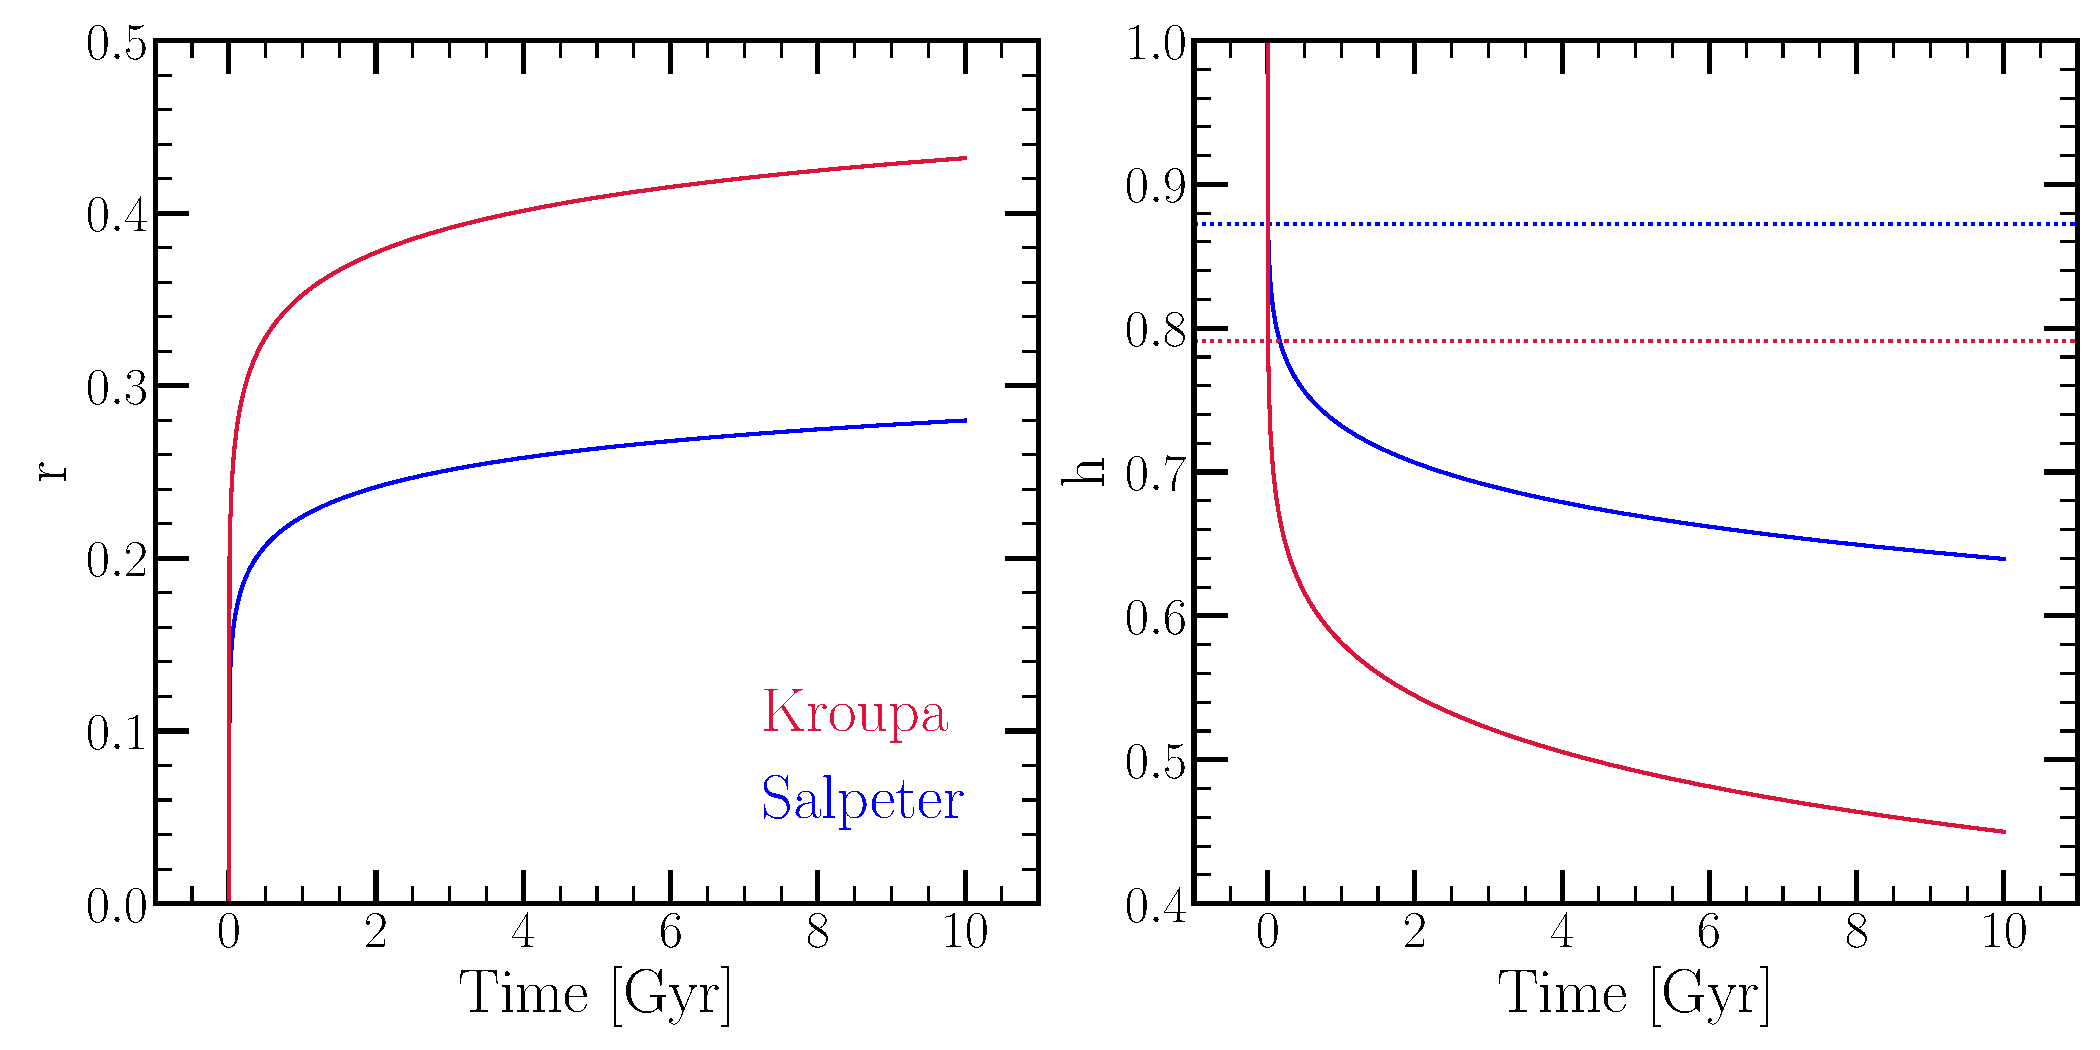
\includegraphics[scale = 0.47]{../rh_2panel/rh2panel.pdf}
\caption{\textbf{Left}: The cumulative return fraction $r(t)$ as implemented 
in \texttt{VICE} for both Kroupa (2001), MNRAS, 322, 231 and Salpeter (1955), 
ApJ, 121, 161 initial mass functions (IMFs). \textbf{Right}: The main sequence 
mass fraction $h(t)$ as implemented in \texttt{VICE} for both Kroupa and 
Salpeter IMFs. The calculations presented in these figures are for lower and 
upper mass limits on star formation of 0.08 and 100 $M_\odot$. After 10 Gyr, 
the approximation $h(t) \approx 1 - r(t)$ fails at the~$\sim$15\% level; thus 
\texttt{VICE} does not adopt such a formalism. } 
\label{fig:rh_2panel}
\end{figure*}

\begin{figure*}[!ht]
\centering
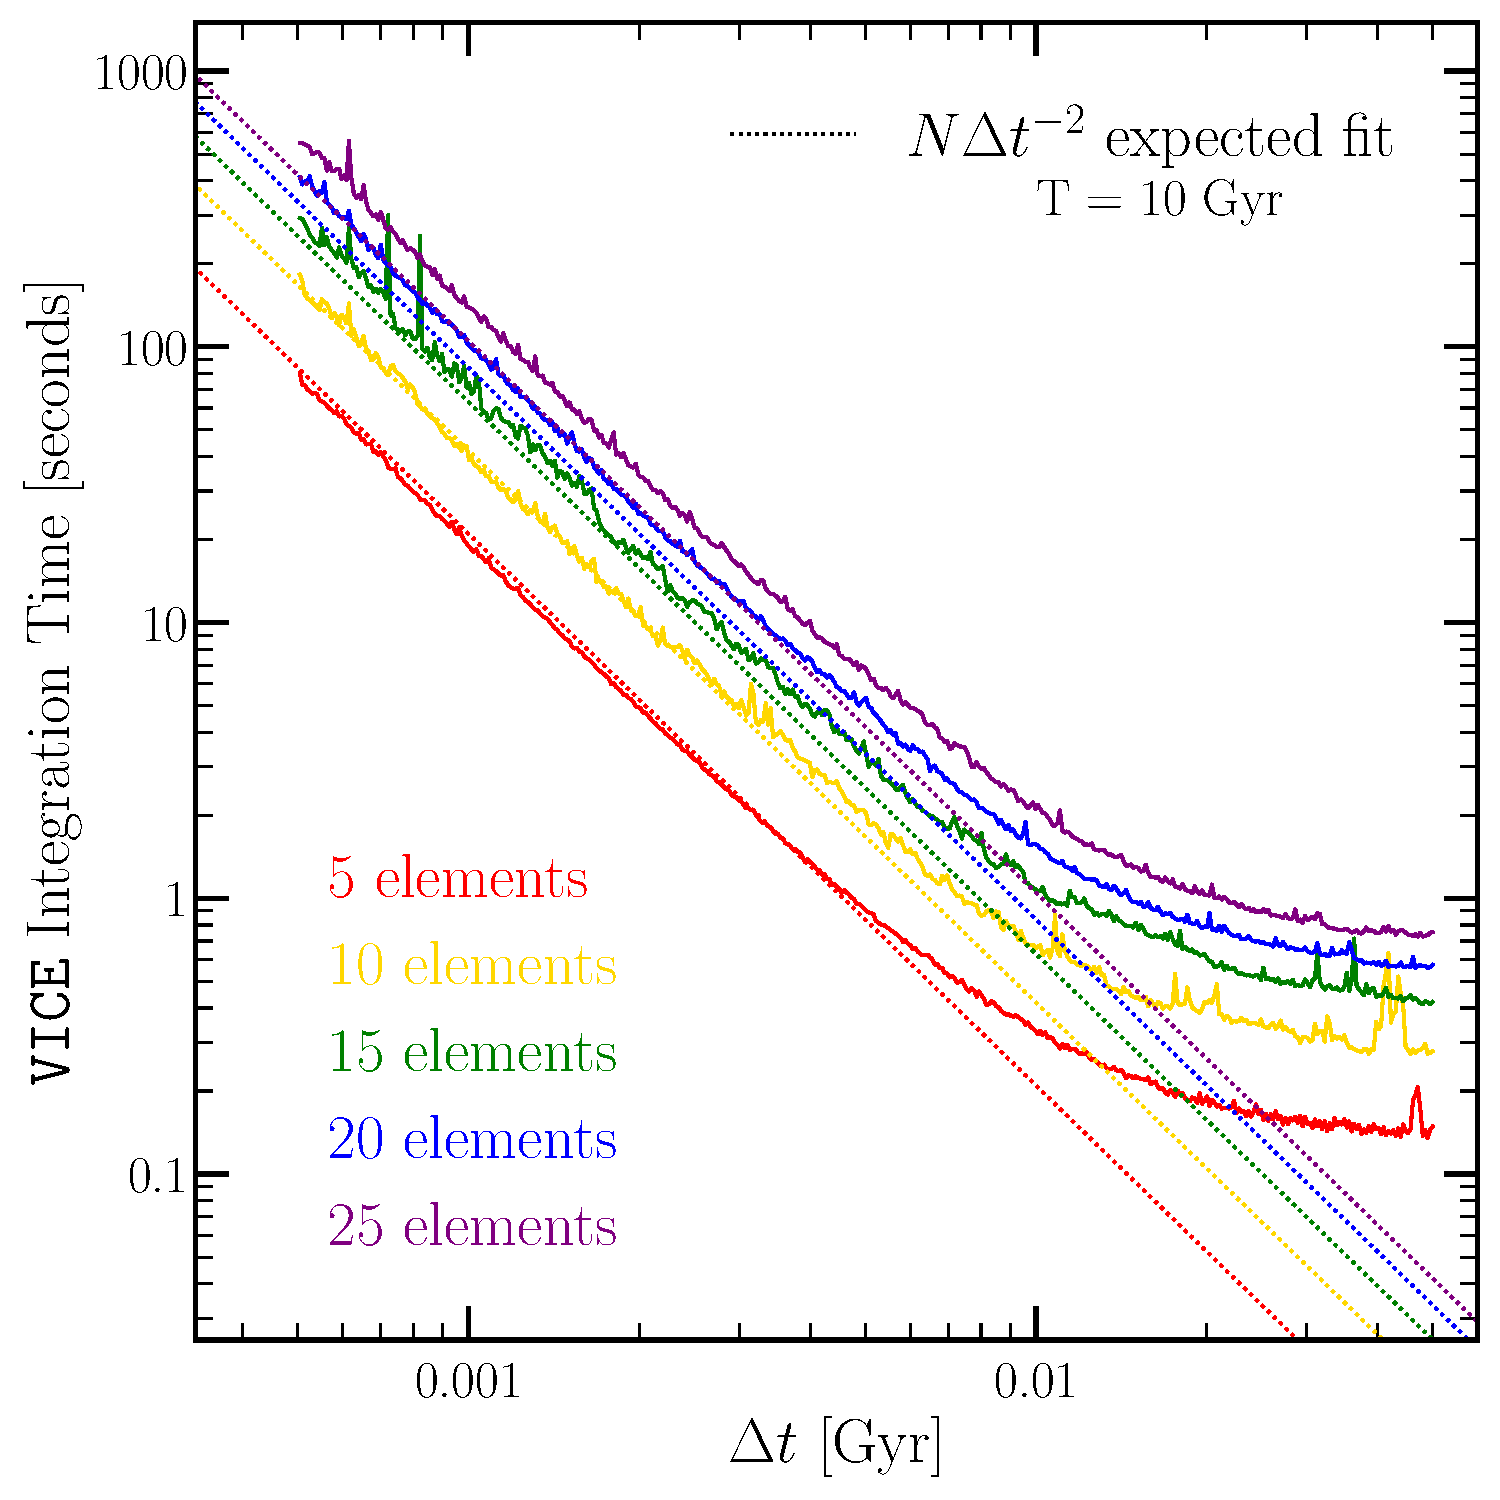
\includegraphics[scale = 0.4]{../timer/timer.pdf}
\caption{Timed runs with $N$ = 5, 10, 15, 20, and 25 elements with timesteps 
ranging from 500 kyr to 10 Myr (solid lines) with an ending time of 
$T$ = 10 Gyr. I overplot the corresponding color-coded dotted lines showing 
the $N\Delta t^{-2}$ expected fit. The fit does well for low $N$, but 
mildly underpredicts the integration time for higher $N$. The deviation from 
the expected fit for coarse timestepping is due to the transition from an 
algorithm-limited simulation to a write-out limited simulation.}
\label{fig:timer}
\end{figure*} 


% \bibliographystyle{mnras}
% \bibliography{science_documentation}

\end{document}

